\pdfoutput=1

\section{Experiments} \label{sec:exp}
% To evaluate the effectiveness and efficiency of \method, we conduct comprehensive experiments to answer the following research questions:\\
% \textbf{RQ1}: Is single-turn \method~better than baselines on both in-distribution and out-of-distribution test sets?\\
% \textbf{RQ2}: Why LLMs need meta-thinking in reasoning during RL training?\\
% \textbf{RQ3}: How well can LLMs learn to meta-think?\\
% \textbf{RQ4}: How does reward functions affect the evolution of the agents during RL training?\\
% \textbf{RQ5}: Can \method~be scaled to multi-turn settings and does it benefit from turn-level ratio?\\

To evaluate the effectiveness and efficiency of \method, we conduct experiments on challenging benchmarks for two types of tasks: mathematical reasoning and LLM-as-a-Judge with three different LLMs. Then, we investigate the models' performance in both single‑ \& multi‑turn settings. Finally, we provide ablation studies and qualitative analyses of our method. 

% We aim to answer the following research questions:
% \begin{itemize}
%     \item \textbf{RQ1}: Does \method~outperform baselines on both in-distribution and out-of-distribution test sets?
%     \item \textbf{RQ2}: Does MAMRP execution facilitate the RL training of the lower-level solving agent $\pi_{\theta_l}$?
%     \item \textbf{RQ3}: How do different reward functions affect \method's performance and LLMs' outputs?
%     \item \textbf{RQ4}: What types of metacognition emerge in \method?
% \end{itemize}



\subsection{Experiment Settings} 
\label{sec:exp_settings}
We first analyze the single-turn case of ReMA, \ie, $T=1$. 
The high-level agent generates a complete meta-thinking trace in one shot, and the low-level agent follows the instructions and outputs the final results. 
Single-turn ReMA reduces stochasticity and training cost while our experiments show that it still provides meaningful performance gains.

\paragraph{Benchmarks} We conduct experiments on two types of tasks: mathematical reasoning and LLM-as-a-Judge. For mathematical reasoning experiments, we train models on 7.5k training samples in MATH \citep{hendrycks2021measuring} and use MATH500 \citep{lightman2023let} as the in-distribution test dataset. Additionally, we test the optimized models on out-of-distribution datasets: GSM8K \citep{cobbe2021training}, AIME24\footnote{\texttt{https://huggingface.co/datasets/AI-MO/aimo-validation-aime}}, AMC23\footnote{\texttt{https://huggingface.co/datasets/AI-MO/aimo-validation-amc}}, GaoKao2023En \citep{zhang2023evaluating}, Minerva Math \citep{lewkowycz2022solving}, and Olympiad Bench \citep{he2024olympiadbench}. 

For LLM-as-a-Judge benchmarks, we train models on RewardBench \citep{lambert2024rewardbench}. Specifically, we convert the original data into a pair-ranking format and split it into a training set of 5k items and a test set of 970 items, denoted as RewardBench970. The models are also tested on JudgeBench \citep{tan2024judgebench} to assess out-of-distribution performance. We refer to Appendix~\ref{app:exp_setting.single_turn_rema.rewardbench970} for detailed comparisons and results.

\paragraph{Baselines, Models, Training Settings} 
We compare pass@1 performance across the following methods:
(1) \textbf{VRP} (CoT, step-by-step prompting, Sec.~\ref{sec:method.reinforce_ma.deploy_ma}); 
(2) \textbf{VRP$_\text{RL}$} (RL under VRP);
(3) \textbf{MRP$_\text{RL}$} (RL under MRP with high-level task analysis, Eq.~(\ref{eq:mcp2})), and (4) \textbf{\method}~(ours, RL under MAMRP, Eq.~(\ref{eq:mamrp2})).
% and the majority voting results under temperature $0.7$. Specifically, for \textit{MAMRP}, we sample multiple $\mathbf{m}$ under temperature $0.7$ and then sample the corresponding $\mathbf{y}$ using greedy decoding.

We train and test Llama-3-8B-Instruct, Llama-3.1-8B-Instruct \citep{dubey2024llama}, and Qwen2.5-7B-Instruct \citep{qwen2.5} on mathematical reasoning benchmarks.
For LLM-as-a-judge benchmarks, we train and test Llama-3.1-8B-Instruct and Qwen2.5-7B-Instruct. 
We use instruct-tuned LLMs to prompt them to perform VRP, MRP, and MAMRP directly during training.
Unless specified, we use two separate copies of the same model for high- and low-level agents in \method.
% Unless specified, we use the same model for \textit{MAMRP} and two separate models trained from the same original model for \method, 
We use the base reward setting in Appendix~\ref{app:reward_design} by default. And for the underlying RL algorithm, we use REINFORCE++ \citep{hu2025reinforce++}. We refer to Appendix~\ref{app:exp_setting} for detailed training settings.

\subsection{Results of Single-turn \method}
\label{sec:exp.single_turn}
\textbf{Question 1.} \textit{Does single-turn \method~outperforms baselines on both in-distribution and out-of-distribution test sets?}

Table~\ref{tab:exp_main} compares the greedy decoding performance of \method~against various RL baselines across mathematical benchmarks (Table~\ref{tab:exp_main.math}) and LLM-as-a-Judge benchmarks (Table~\ref{tab:exp_main.laaj}). Results across different LLMs indicate that, \textbf{on average, \method~outperforms all baselines}, achieving a maximum improvement of 6.68\% on mathematical benchmarks and 8.49\% on LLM-as-a-Judge benchmarks.

Notably, \method~achieves the highest performance on most benchmarks, particularly on out-of-distribution datasets, with a maximum improvement of 20\% on AMC23 for Llama3-8B-Instruct, 13.33\% on AIME24 for Qwen2.5-7B-Instruct, 14.23\% on RewardBench970 for Llama3.1-8B-Instruct. 
These results demonstrate the superior out-of-distribution generalization ability conferred by the meta-thinking mechanism in \method.
However, we observe that the accuracy gains from RL training on instruction-tuned LMs are smaller than from base models (Sec.~\ref{sec:exp.low_rl}).
This may be due to the higher initial performance and the relatively fixed output distribution of instruction-tuned models, which limits the improvement and peak performance in RL.

\definecolor{DarkGreen}{RGB}{0,100,0} % Dark green for better readability
\definecolor{InDist}{RGB}{220, 240, 255}  % Light blue
\definecolor{OutDist}{RGB}{255, 230, 230} % Light red
\definecolor{DarkRed}{RGB}{139, 0, 0} % Dark red
\begin{table}[t]
    \small
    \centering
    \caption{Performance on \colorbox{InDist}{in-distribution} test sets and \colorbox{OutDist}{out-of-distribution} test sets.
    We also report the \textcolor{red}{improvement}/\textcolor{DarkGreen}{degradation} w.r.t. basic CoT performance(VRP). On average, \method~outperforms all
baselines. Particularly on out-of-distribution datasets, \method~achieves the highest performance on most of the benchmarks.}
    \label{tab:exp_main}
    \vspace{-5pt}
    \begin{subtable}{\linewidth}
        \centering
        \caption{Performance on math benchmarks}
        \label{tab:exp_main.math}
        \vspace{-5pt}
        \begin{tabular}{c||c|cccc}
            % \multicolumn{5}{c}{\textbf{Llama3-8B-Instruct}}\\
            \toprule
            \textbf{Model} & \textbf{Benchmark} & \makecell{\textbf{VRP}\\(CoT)} & \textbf{VRP$_\text{RL}$} & \textbf{MRP$_\text{RL}$ }& \makecell{\textbf{\method}\\(Ours)} \\ 
            \toprule
            
            \multirow{8}{*}{\textbf{\makecell{Llama3\\-8B\\-Instruct}}} & \cellcolor{InDist} MATH500 & 30.80 & 33.40 (\textcolor{red}{+2.60}) & 32.80 (\textcolor{red}{+2.00}) & \textbf{33.80 (\textcolor{red}{+3.00})} \\
    & \cellcolor{OutDist} GSM8K & 67.48 & \textbf{81.80 (\textcolor{red}{+14.32})} & 79.68 (\textcolor{red}{+12.20}) & 79.38 (\textcolor{red}{+11.90}) \\
    & \cellcolor{OutDist} AIME24 & 0.00 & 0.00 (\textcolor{DarkGreen}{+0.00}) & \textbf{3.33 (\textcolor{red}{+3.33})} & 0.00 (\textcolor{DarkGreen}{+0.00}) \\
    & \cellcolor{OutDist} AMC23 & 2.50 & 10.00 (\textcolor{red}{+7.50}) & 12.50 (\textcolor{red}{+10.00}) & \textbf{22.50 (\textcolor{red}{+20.00})} \\
    & \cellcolor{OutDist} Gaokao2023en & 22.34 & 27.53 (\textcolor{red}{+5.19}) & 23.38 (\textcolor{red}{+1.04}) & \textbf{28.57 (\textcolor{red}{+6.23})} \\
    & \cellcolor{OutDist} Minerva Math & 8.82 & 16.54 (\textcolor{red}{+7.72}) & \textbf{18.01 (\textcolor{red}{+9.19})} & 13.97 (\textcolor{red}{+5.15}) \\
    & \cellcolor{OutDist} Olympiad Bench & 8.44 & 8.89 (\textcolor{red}{+0.45}) & \textbf{9.33 (\textcolor{red}{+0.89})} & 8.89 (\textcolor{red}{+0.45}) \\
    \cmidrule{2-6}
    & Average & 20.05 & 25.45 (\textcolor{red}{+5.40}) & 25.58 (\textcolor{red}{+5.53}) & \textbf{26.73 (\textcolor{red}{+6.68})} \\
            \toprule
            \multirow{8}{*}{\textbf{\makecell{Llama3.1\\-8B\\-Instruct}}} 
            & \cellcolor{InDist} MATH500 & 50.80 & 50.20 (\textcolor{DarkGreen}{-0.60}) & 48.60 (\textcolor{DarkGreen}{-2.20}) & \textbf{53.20 (\textcolor{red}{+2.40})} \\
    & \cellcolor{OutDist} GSM8K & 86.05 & 84.53 (\textcolor{DarkGreen}{-1.52}) & 85.37 (\textcolor{DarkGreen}{-0.68}) & \textbf{87.26 (\textcolor{red}{+1.21})} \\
    & \cellcolor{OutDist} AIME24 & 10.00 & 3.33 (\textcolor{DarkGreen}{-6.67}) & 6.67 (\textcolor{DarkGreen}{-3.33}) & \textbf{13.33 (\textcolor{red}{+3.33})} \\
    & \cellcolor{OutDist} AMC23 & 27.50 & 12.50 (\textcolor{DarkGreen}{-15.00}) & \textbf{30.00 (\textcolor{red}{+2.50})} & 20.00 (\textcolor{DarkGreen}{-7.50}) \\
    & \cellcolor{OutDist} Gaokao2023en & \textbf{38.96} & 36.10 (\textcolor{DarkGreen}{-2.86}) & 37.14 (\textcolor{DarkGreen}{-1.82}) & 37.14 (\textcolor{DarkGreen}{-1.82}) \\
    & \cellcolor{OutDist} Minerva Math & 22.79 & 26.84 (\textcolor{red}{+4.05}) & 25.37 (\textcolor{red}{+2.58}) & \textbf{28.31 (\textcolor{red}{+5.52})} \\
    & \cellcolor{OutDist} Olympiad Bench & 15.11 & \textbf{19.70 (\textcolor{red}{+4.59})} & 15.70 (\textcolor{red}{+0.59}) & 19.56 (\textcolor{red}{+4.45}) \\
    \cmidrule{2-6}
    & Average & 35.89 & 33.32 (\textcolor{DarkGreen}{-2.57}) & 35.55 (\textcolor{DarkGreen}{-0.34}) & \textbf{36.97 (\textcolor{red}{+1.08})} \\
            \toprule        
            \multirow{8}{*}{\textbf{\makecell{Qwen2.5\\-7B\\-Instruct}}} & \cellcolor{InDist} MATH500 & 75.00 & \textbf{77.20 (\textcolor{red}{+2.20})} & 76.40 (\textcolor{red}{+1.40}) & 74.40 (\textcolor{DarkGreen}{-0.60}) \\
    & \cellcolor{OutDist} GSM8K & \textbf{92.04} & 91.36 (\textcolor{DarkGreen}{-0.68}) & 91.81 (\textcolor{DarkGreen}{-0.23}) & 90.60 (\textcolor{DarkGreen}{-1.44}) \\
    & \cellcolor{OutDist} AIME24 & 6.67 & 6.67 (\textcolor{DarkGreen}{+0.00}) & 10.00 (\textcolor{red}{+3.33}) & \textbf{20.00 (\textcolor{red}{+13.33})} \\
    & \cellcolor{OutDist} AMC23 & 47.50 & 50.00 (\textcolor{red}{+2.50}) & 52.50 (\textcolor{red}{+5.00}) & \textbf{57.50 (\textcolor{red}{+10.00})} \\
    & \cellcolor{OutDist} Gaokao2023en & 56.62 & 54.81 (\textcolor{DarkGreen}{-1.81}) & 55.06 (\textcolor{DarkGreen}{-1.56}) & \textbf{57.92 (\textcolor{red}{+1.30})} \\
    & \cellcolor{OutDist} Minerva Math & \textbf{35.66} & 34.93 (\textcolor{DarkGreen}{-0.73}) & 32.35 (\textcolor{DarkGreen}{-3.31}) & 34.93 (\textcolor{DarkGreen}{-0.73}) \\
    & \cellcolor{OutDist} Olympiad Bench & 38.22 & \textbf{38.37 (\textcolor{red}{+0.15})} & 37.78 (\textcolor{DarkGreen}{-0.44}) & 36.30 (\textcolor{DarkGreen}{-1.92}) \\
    \cmidrule{2-6}
    & Average & 50.24 & 50.48 (\textcolor{red}{+0.24}) & 50.84 (\textcolor{red}{+0.60}) & \textbf{53.09 (\textcolor{red}{+2.85})} \\
            \bottomrule
        \end{tabular}
    \end{subtable}
    
    \vspace{-1pt}
    \begin{subtable}{\linewidth}
        \centering
        \caption{Performance on LLM-as-a-Judge benchmarks}
        \label{tab:exp_main.laaj}
        \vspace{-5pt}
        \begin{tabular}{c||c|cccc}
        % \multicolumn{5}{c}{\textbf{Llama3-8B-Instruct}}\\
        \toprule
        \textbf{Model} & \textbf{Benchmark} & \makecell{\textbf{VRP}\\(CoT)} & \textbf{VRP$_\text{RL}$} & \textbf{MRP$_\text{RL}$ }& \makecell{\textbf{\method}\\(Ours)} \\ 
        \toprule
        \multirow{3}{*}{\textbf{\makecell{Llama3.1\\-8B\\-Instruct}}}
        & \cellcolor{InDist} RewardBench970 & 69.48 & 82.89 (\textcolor{red}{+13.41}) & 81.13 (\textcolor{red}{+11.65}) & \textbf{83.71 (\textcolor{red}{+14.23})} \\
& \cellcolor{OutDist} JudgeBench & 51.29 & 51.94 (\textcolor{red}{+0.65}) & \textbf{52.90 (\textcolor{red}{+1.61})} & \textbf{52.90 (\textcolor{red}{+1.61})} \\
\cmidrule{2-6}
& Average & 60.39 & 67.41 (\textcolor{red}{+7.02}) & 67.02 (\textcolor{red}{+6.63}) & \textbf{68.31 (\textcolor{red}{+7.92})} \\
\cmidrule{2-6}
% & Average & 61.51 & 66.65 (\textcolor{red}{+5.14}) & 65.53 (\textcolor{red}{+4.02}) & \textbf{70.00 (\textcolor{red}{+8.49})} \\ 
        \toprule        
        \multirow{3}{*}{\textbf{\makecell{Qwen2.5\\-7B\\-Instruct}}}
        & \cellcolor{InDist} RewardBench970 & 78.56 & 85.36 (\textcolor{red}{+6.80}) & \textbf{86.49 (\textcolor{red}{+7.93})} & 83.51 (\textcolor{red}{+4.95}) \\
& \cellcolor{OutDist} JudgeBench & \textbf{58.39} & 56.94 (\textcolor{DarkGreen}{-1.45}) & 58.39 (\textcolor{DarkGreen}{+0.00}) & 56.94 (\textcolor{DarkGreen}{-1.45}) \\
\cmidrule{2-6}
& Average & 68.47 & 71.15 (\textcolor{red}{+2.68}) & \textbf{72.44 (\textcolor{red}{+3.97})} & 70.22 (\textcolor{red}{+1.75}) \\
        \bottomrule
    \end{tabular}
\end{subtable}
\vspace{-10pt}
\end{table}

% Beyond the higher initial performance of instruction-tuned models, we hypothesize that this is due to their relatively fixed output distribution, which limits their adaptability and exploration in reinforcement learning. Additionally, the relatively small model size and dataset scale may further constrain the improvements achieved through reinforcement learning. 
% We are actively scaling our approach to larger models and datasets to further investigate these limitations.

% \subsubsection{Ablations}
%\subsubsection{Given meta-thougts generated in MAMRP, low-level solving agent $\pi_{\theta_l}$ generalizes best during RL training. \ying{it is a conclusion, not a sub section name?}}\hj{Meta-thoughts boost low-level generalization}
\subsubsection{Meta-thoughts boost low-level generalization}
\label{sec:exp.low_rl}
\begin{figure}[t]
    \vspace{-10pt}
    \centering
    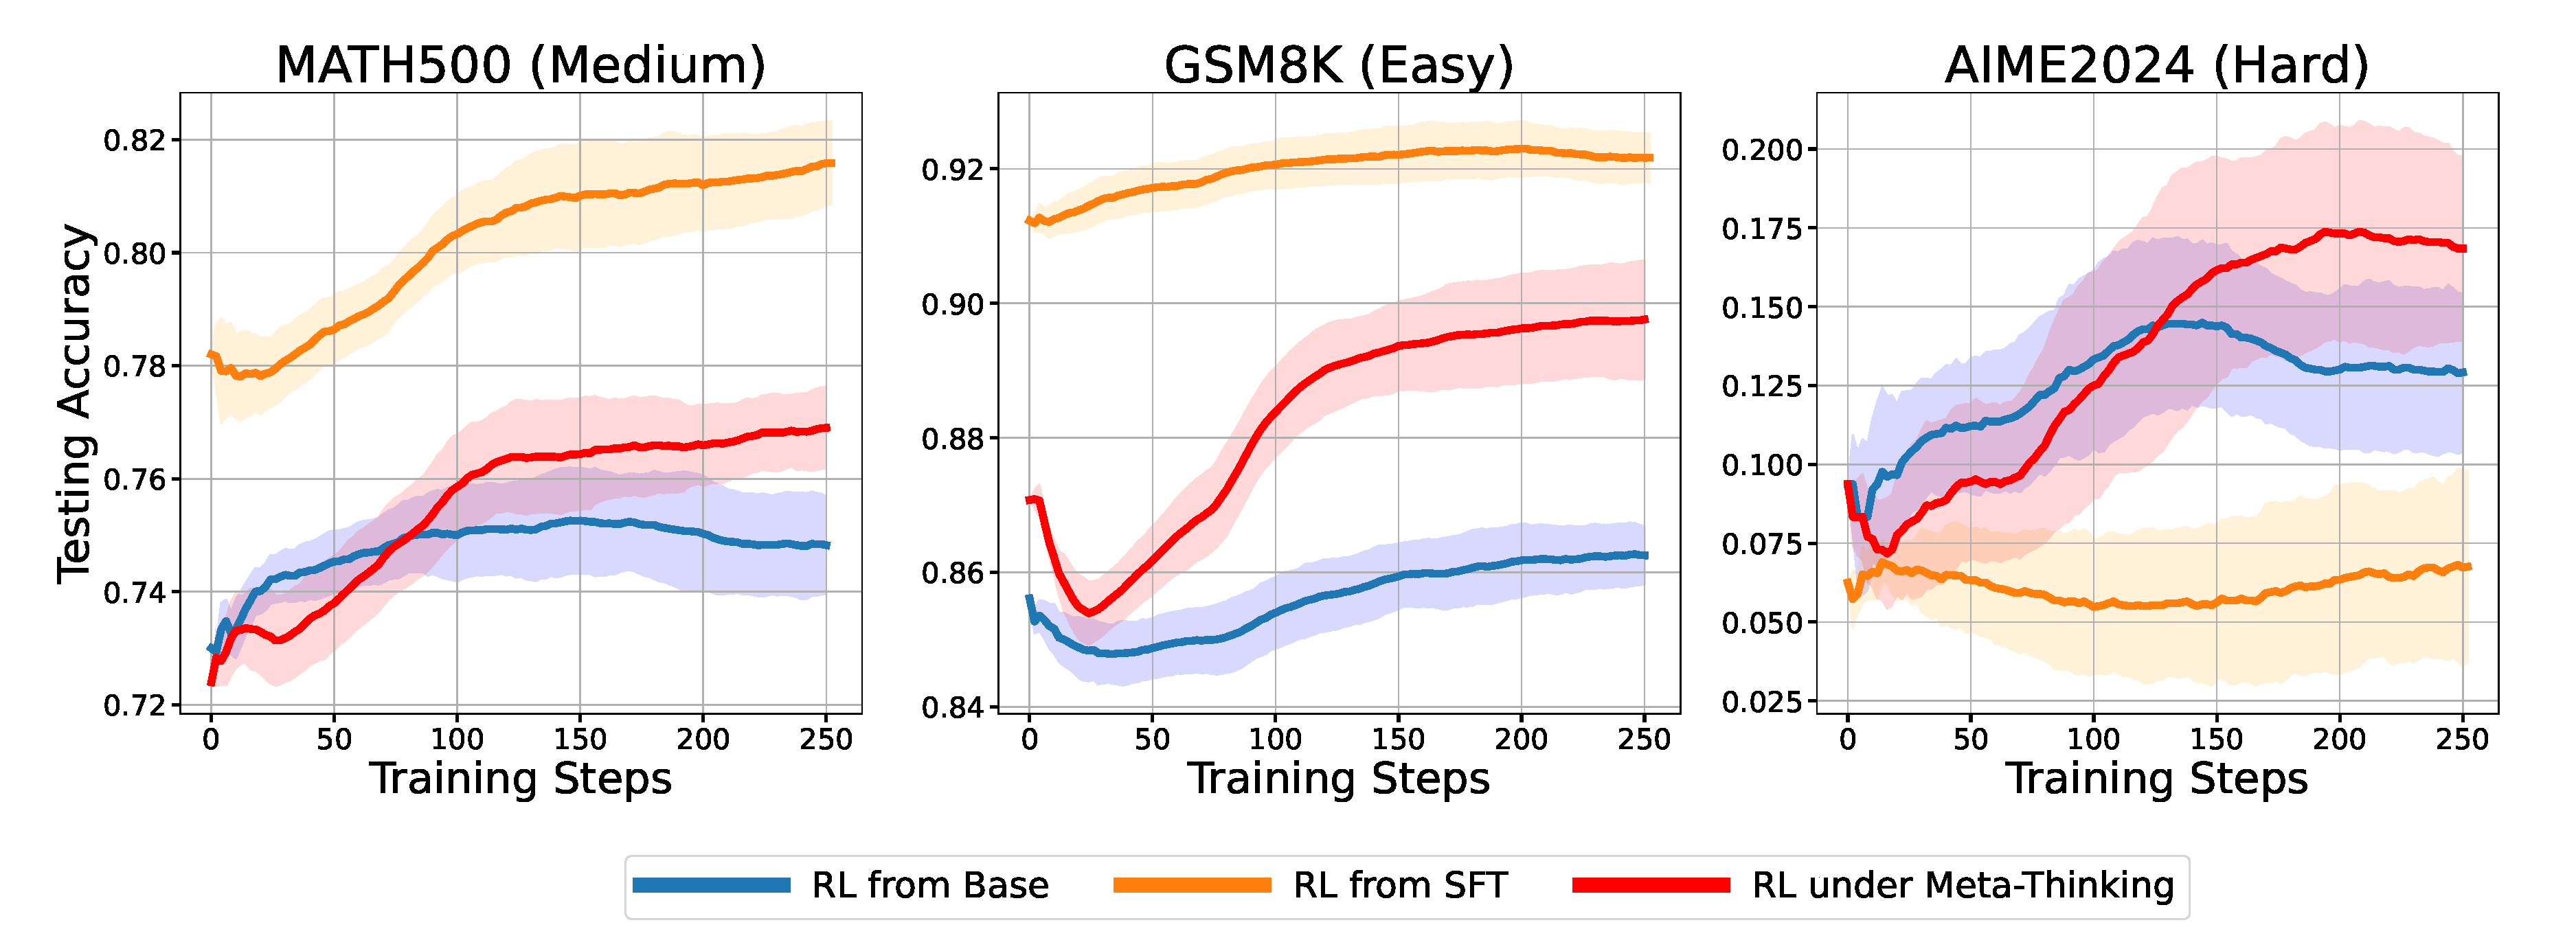
\includegraphics[width=\linewidth]{figures/compare_rl_acc_only.pdf}
    \vspace{-10pt}
    \caption{
        % The performance of Qwen2.5-Math-7B on the MATH500, GSM8K, and AIME24 datasets during RL training on Level 3-5 MATH questions under different training schemes. \textbf{RL from SFT} achieves superior performance but struggles to generalize to more challenging problems. In contrast, \textbf{RL from Base} and \textbf{RL under Meta-thinking} demonstrate the ability to solve previously unseen, harder problems, with the latter further enhancing performance.
        An RL experiment with 3 training schemes. While \textbf{RL from SFT} excels on easier problems, \textbf{RL under Meta-thinking} shows superior generalization to harder problems like AIME24.
        }
        \label{fig:compare_rl}
        \vspace{-10pt}
\end{figure}
\textbf{Question 2.} \textit{Can Reasoning benefit from Meta-thinking?}

Here we provide a tiny but motivating example of how \method~gives better learning dynamics. We use Qwen2.5-Math-7B \citep{yang2024qwen25mathtechnicalreportmathematical} as the starting base model, MATH (level 3-5, about 5.5K number of instances) as the training dataset, and we compare three reinforcement learning training schemes, in particular:
(1) \textbf{RL from Base}: train the base model directly on MATH with binary outcome reward;
(2) \textbf{RL from SFT}: SFT the base model with GPT-4o's CoT answers; then RL on train dataset with binary outcome reward;
(3) \textbf{RL under Meta-thinking}: SFT the base model with GPT-4o's meta-thinking plans; then RL on train dataset with binary outcome reward.
    % \begin{enumerate}
%     \item \textbf{RL from Base}: train the base model directly on MATH with binary outcome reward;
%     % \item \textbf{RL from SFT}: First, collect a small amount of CoT data (from GPT-4o's answers) to fine-tune the base model (SFT); then train the tuned model on MATH with binary outcome reward;
%     \item \textbf{RL from SFT}: SFT the base model with GPT-4o's CoT answers; then RL on train dataset with binary outcome reward;
%     % \item \textbf{RL under Meta-thinking}: First, collect a small amount of high-level meta-thinking data (from GPT-4o's plans) to fine-tune Qwen2.5-Math-7B-Instruct \citep{yang2024qwen25mathtechnicalreportmathematical} to increase its meta-thinking abilities and make sure it act as high-level planner only; then train Qwen2.5-Math-7B as the low-level agent in collaboration with the high-level instruction with binary outcome reward.
%     \item \textbf{RL under Meta-thinking}: SFT the base model with GPT-4o's meta-thinking plans; then RL on train dataset with binary outcome reward.
% \end{enumerate}
% The model is tested on a testing set of MATH500, GSM8K, and AIME24. The results are shown in Figure \ref{fig:compare_rl}. First, supervised fine-tuning (SFT) largely boosts performance as it has the best accuracy on the in-distribution test set MATH500 and the easier one GSM8K at the beginning of RL training. However, it doesn't show advances on the harder benchmark AIME24.
% More importantly, while \textbf{RL from SFT} significantly boosts performance, it struggles to generalize to harder problems. In contrast, \textbf{RL from Base} shows limited improvements, especially on more challenging tasks. 
% Notably, \textbf{RL under Meta-thinking achieves the best learning dynamics, effectively leveraging high-level guidance to improve the performance of the lower-level solving agent}, particularly on harder problems like AIME2024. 
% We refer to Appendix~\ref{app:qualitative_results.high_level_better} for case study.

The models are evaluated on 3 benchmarks (Fig.~\ref{fig:compare_rl}). SFT brings the best initial accuracy on in-distribution and easier sets, but fails to improve on harder ones. \textbf{RL from Base} yields limited gains. In contrast, \textbf{RL under Meta-thinking achieves the best learning dynamics and generalizes better to challenging problems} (AIME24). 
See Appendix~\ref{app:qualitative_results.high_level_better} for case studies.

%\subsubsection{Different reward function designs can encourage different interaction patterns in MAMRP \ying{it is a conclusion, not a sub section name?}\yly{Agree. Need to change.}}\hj{Reward functions shape cross-agent behaviors}


%\subsection{Different LLMs learn various meta-thinking behaviors.}\hj{Diverse meta-thinking characteristics of LLMs}
\subsubsection{Diverse meta-thinking characteristics of LLMs}
\label{sec:exp.high_rl}

\textbf{Question 3.} \textit{How well can LLMs learn to meta-think?}

To further analyze meta-thinking behaviors, we train models with structured JSON-format actions inspired by \citet{yuedots}. The meta-thinking agent generate two entries in one LM call, first selects from three actions: \texttt{DECOMPOSE} (breaking into subproblems), \texttt{REWRITE} (simplifying the problem), or \texttt{EMPTY} (direct solving), then generates the corresponding text.
% We compare two experimental setups using Llama-3.1-8B-Instruct and Llama-3.2-1B-Instruct.  
% These configurations allow us to study models of different scales: one setup consists of two 1B models, while the other consists of two 8B models.  
% This setup enables us to investigate the impact of RL on the final training results of the high-level agent.  
% To ensure the model maintains valid output formatting, we employ {VLLM guided JSON decoding} \citep{kwon2023efficient,dong2024xgrammar} during rollout.  
% We use the base reward setting, \ie, the averaged accuracy of the low-level agent's solutions with format constraints.  
We compare Llama-3.1-8B-Instruct and Llama-3.2-1B-Instruct to study scale effects (two 1B models vs two 8B models) on meta-thinking agent's training. We use vLLM guided JSON decoding \citep{dong2024xgrammar} for valid formatting and base reward (reasoning agent's solution accuracy with format constraints).

% First, we observe that the outputs of smaller language models (LMs) tend to converge to relatively simpler and shorter sentences compared to those in our main experiments. This may be due to the limited capacity of smaller LMs to generate valid JSON-formatted responses while simultaneously exploring diverse reasoning strategies.
% As shown in Fig.~\ref{fig:exp_absl_json}, Llama-3.2-1B-Instruct struggles to capture the complex dynamics underlying the task. Instead, it quickly converges to outputting only the \texttt{EMPTY} action to minimize penalties associated with formatting errors.
% In contrast, Llama-3.1-8B-Instruct successfully learns to employ different metacognitive strategies based on the difficulty level of the problem. A detailed case study is provided in Appendix~\ref{app:qualative_results.case_study.json}.
We observe that smaller LMs produce simpler outputs, likely due to limited capacity to maintain valid JSON formatting while exploring diverse reasoning strategies. 
As Fig.~\ref{fig:exp_absl_json} shows, smaller LMs like Llama-3.2-1B-Instruct quickly converge to the simplest \texttt{EMPTY} action to avoid formatting penalties, \textbf{while larger LMs like Llama-3.1-8B-Instruct can adapt meta-thinking strategies based on problem difficulty}. 
See Appendix~\ref{app:qualative_results.case_study.json} for detailed case studies.

\vspace{-5pt}
\begin{figure}[t]
    \centering
    \begin{subfigure}{0.48\linewidth}
        \centering
        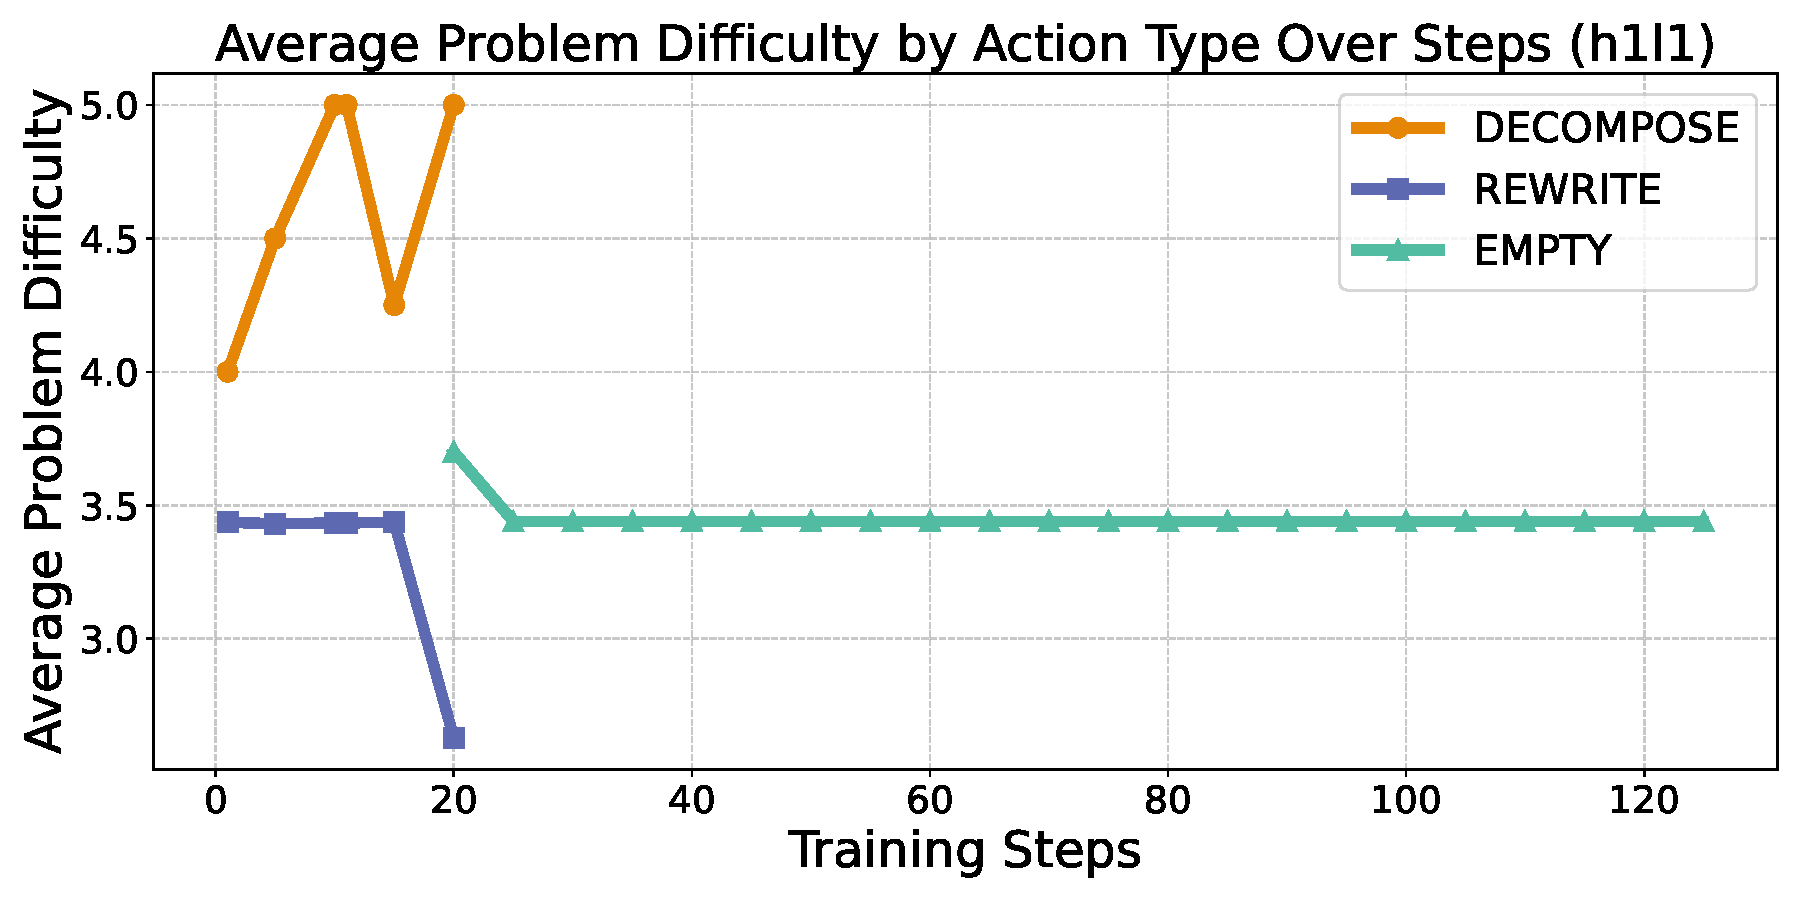
\includegraphics[width=\linewidth]{figures/ablations/difficulty_trends_h1.pdf}
        % \caption{Caption for second image}
        % \label{fig:image2}
    \end{subfigure}
    \hfill
    \begin{subfigure}{0.48\linewidth}
        \centering
        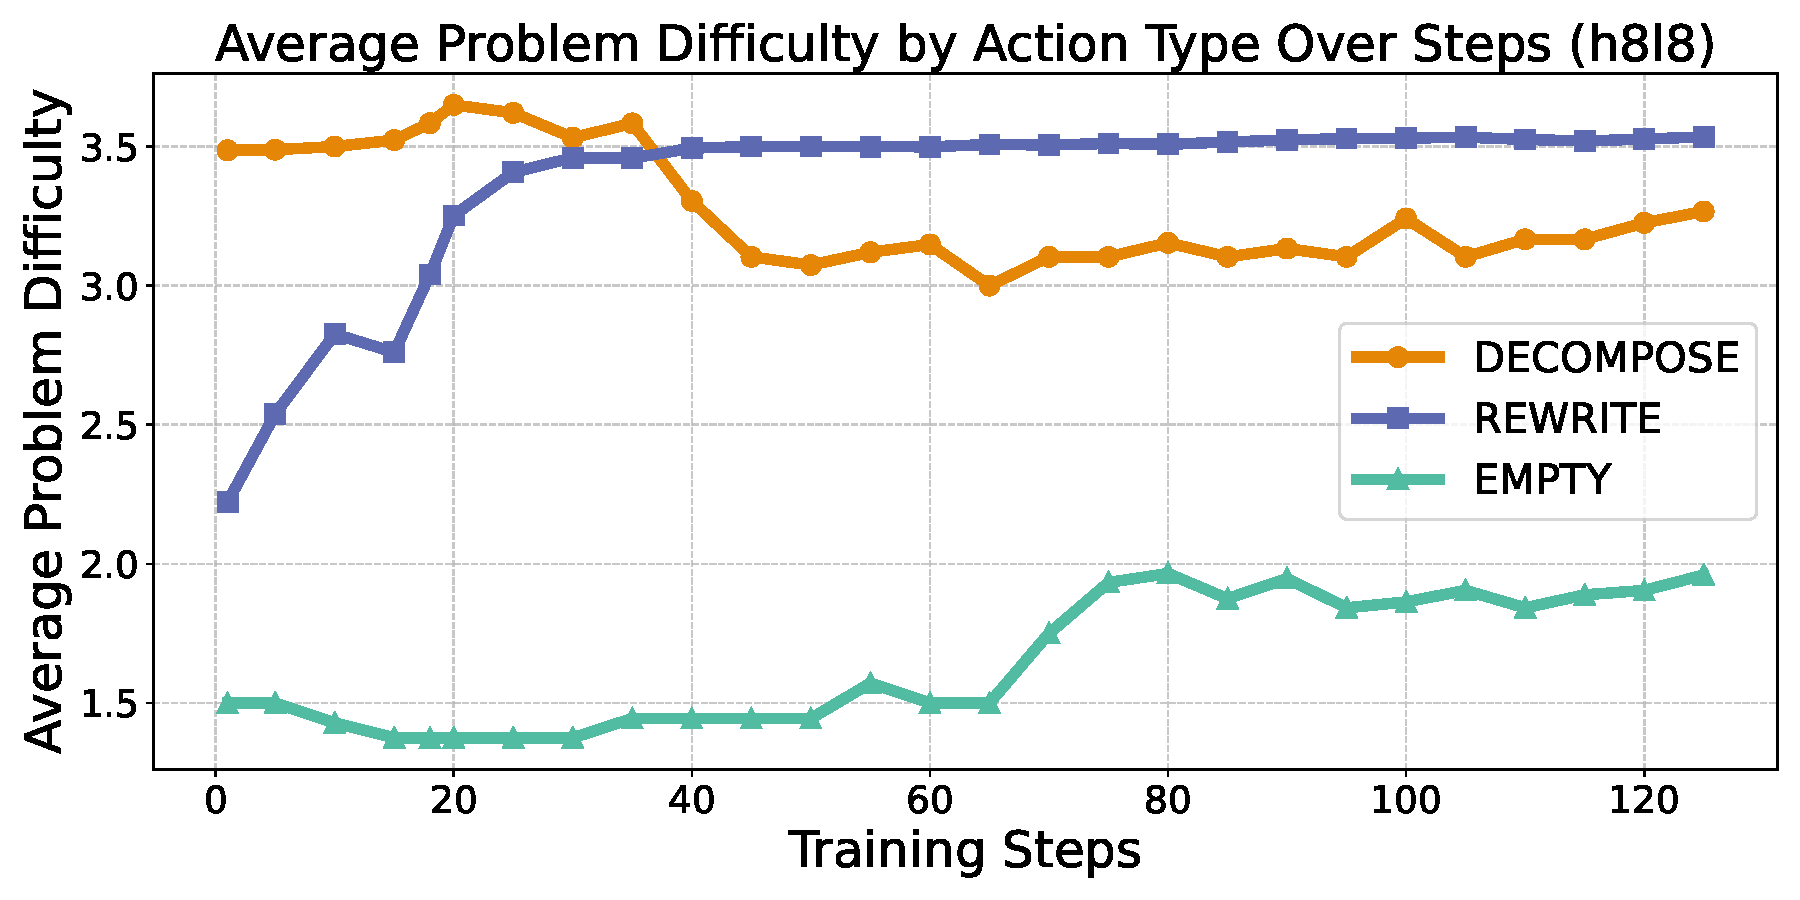
\includegraphics[width=\linewidth]{figures/ablations/difficulty_trends_h8l8.pdf}
        % \label{fig:image1}
    \end{subfigure}
    \vspace{-5pt}
    \caption{
        % Average problem difficulty of three predefined metacognitive actions during training.  
        % \textbf{Left:} After approximately 20 training steps, the 1B LM's outputs collapse to the simplest action, \texttt{EMPTY}, resulting in no data points for \texttt{REWRITE} and \texttt{DECOMPOSE} in the plot.  
        % \textbf{Right:} In contrast, the 8B LM learns to utilize more complex metacognitive actions for solving difficult problems.
        Average problem difficulty by action type during training. \textbf{Left}: 1B LM collapses to the \texttt{EMPTY} action. \textbf{Right}: 8B LM adapts to a more complex meta-thinking strategy for harder problems.
    }
    \label{fig:exp_absl_json}
    \vspace{-10pt}
\end{figure}

\subsection{Extending \method~to Multi-turn MAMRP}
\label{sec:exp.multiturn}

We further extend \method~to multi-turn MAMRP settings, enabling multiple rounds of interaction between the meta-thinking agent and the reasoning agent as defined in Eq.~(\ref{eq:mamrp2}).

% \paragraph{Experimental Setup}
% We evaluate the performance on MATH500 (in-distribution) and out-of-distribution mathematical benchmarks including GSM8K, AIME2024, AIME2025, AMC23, Gaokao2023en, Minerva Math, and Olympiad Bench.
% For model training, we use Qwen2.5-7B and bootstrap the training process with supervised fine-tuning (SFT) data to establish initial multi-turn interaction capabilities. 
% The SFT data consists of 0.8K samples derived from LIMO \citep{ye2025limo}, transformed into multi-turn MAMRP format using GPT-4o.
Unlike the inherent VRP capabilities of most LLMs, multi-turn ReMA requires initial bootstrapping. 
Thus, we constructed a supervised fine-tuning dataset (about 0.8K samples) from LIMO \citep{ye2025limo} using GPT-4o to establish the starting point for multi-turn interaction capabilities. Then we finetune Qwen2.5-7B before RL training. 

As described in Sec.\ref{sec:method.reinforce_ma.multi_turn}, we deploy the proposed GRPO with turn-level ratio clipping and trajectory-level averaging loss during training. 
And we remove the KL-divergence term to allow more flexible exploration.
By default, the agents share the same parameters and are simultaneously updated using their trajectories. We refer to details in Appendix~\ref{app:exp_setting.multi_turn_rema}.

\begin{figure}[t]
    \vspace{-10pt}
    \centering
    \begin{minipage}{0.45\linewidth}
    % \begin{figure}[H]
        \centering
        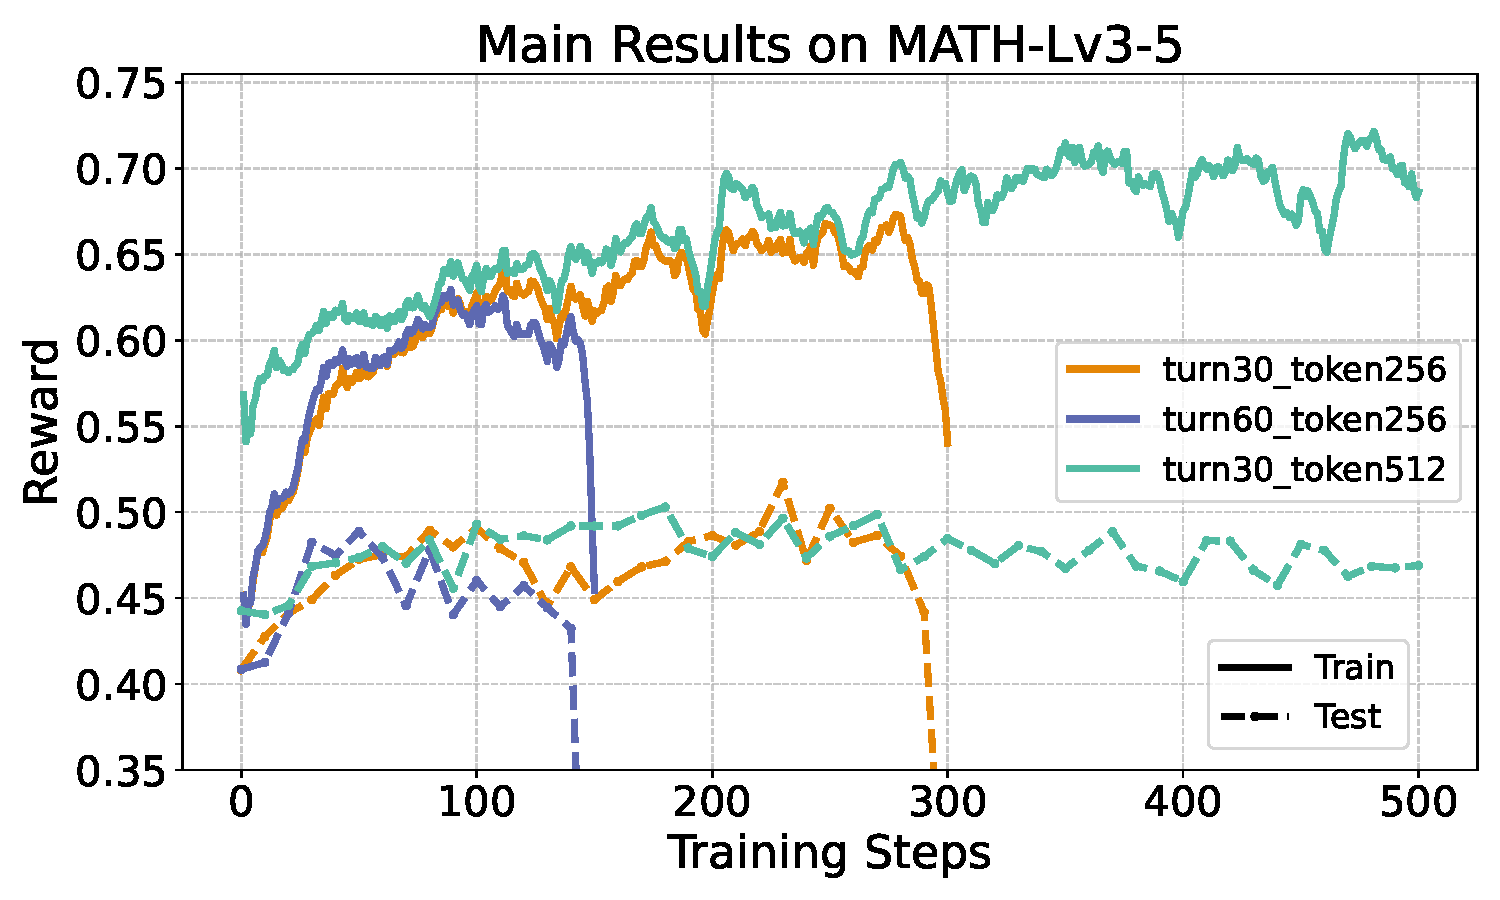
\includegraphics[width=\linewidth]{figures/multi_turn/multi_turn_main.pdf}
        \vspace{-15pt}
        \captionof{figure}{Training results of multi-turn ReMA on MATH-Level3-5-8K under different rollout configurations.}
        \label{fig:multi_turn_main}
    % \end{figure}
    \end{minipage}
    \hfill
    \begin{minipage}{0.54\linewidth}
    % \begin{figure}[H]
        \centering
        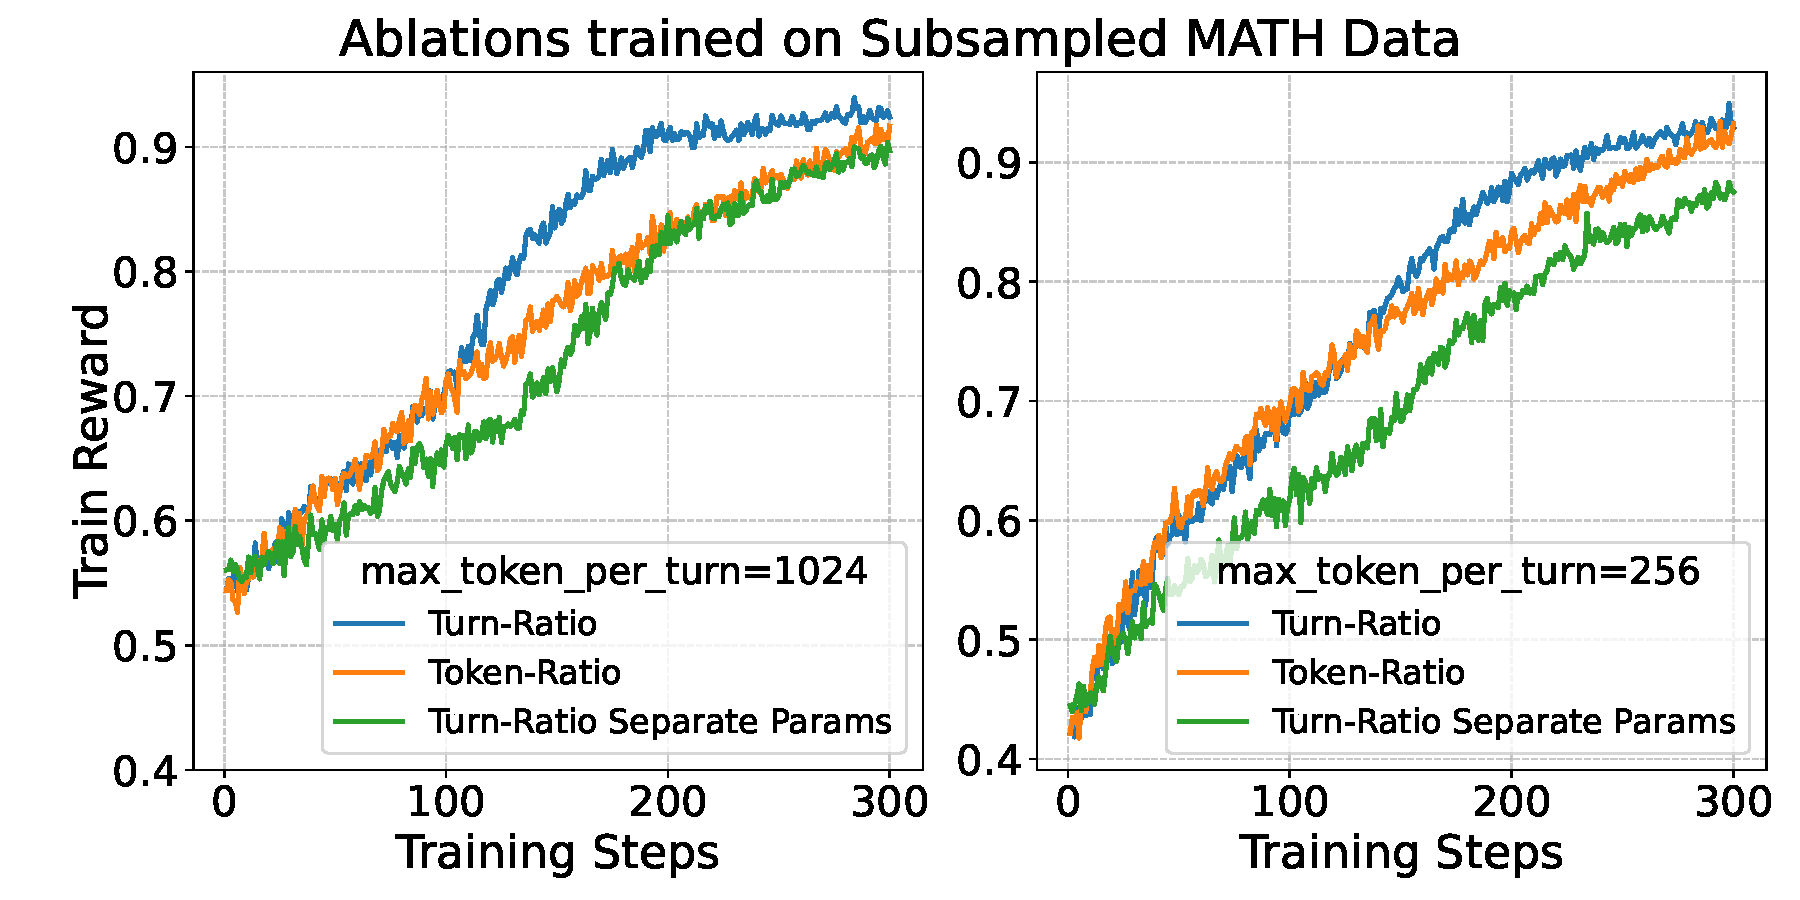
\includegraphics[width=\linewidth]{figures/multi_turn/multi_turn_ablation.pdf}
        \vspace{-15pt}
        \captionof{figure}{Ablations of multi-turn ReMA on a tiny subset of MATH, we only show here the training curves of different training and rollout configurations.}
        \label{fig:multi_turn_ablation}
    % \end{figure}
    \end{minipage}
    \vspace{-10pt}
\end{figure}
% \begin{figure}[t]
%     \begin{subfigure}{0.48\linewidth}
%         \centering
%         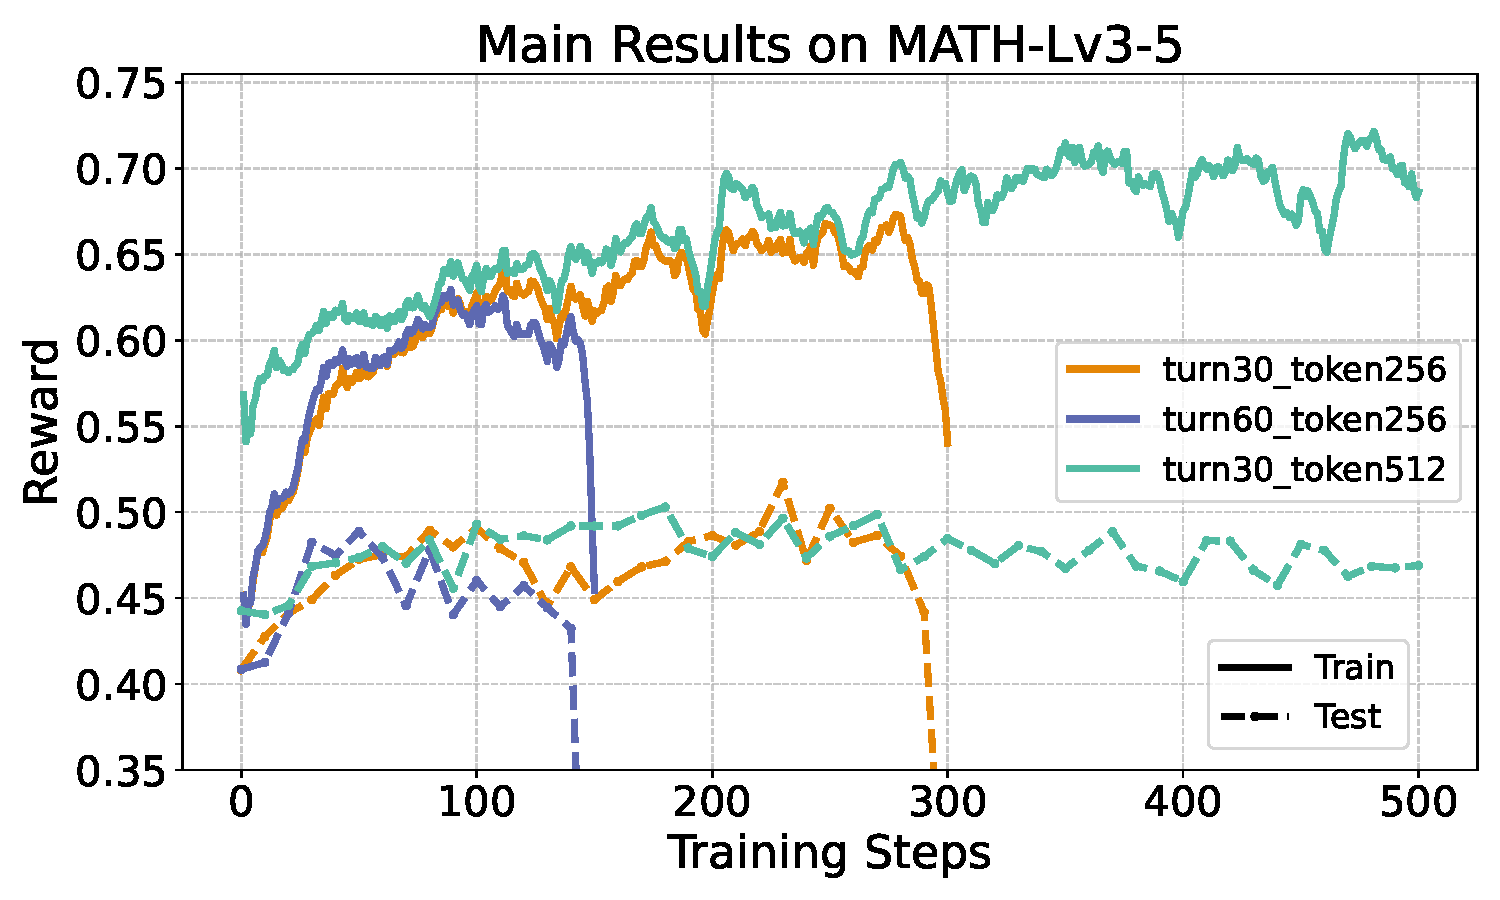
\includegraphics[width=\linewidth]{figures/multi_turn/multi_turn_main.pdf}
%         \vspace{-10pt}
%         \caption{Training results of multi-turn ReMA on MATH-Level3-5-8K, we also show test accuracy averaged over harder test sets mentioned in experimental setup.}
%         \label{fig:multi_turn_main}
%     \end{subfigure}
%     \hfill
%     \begin{subfigure}{0.48\linewidth}
%         \centering
%         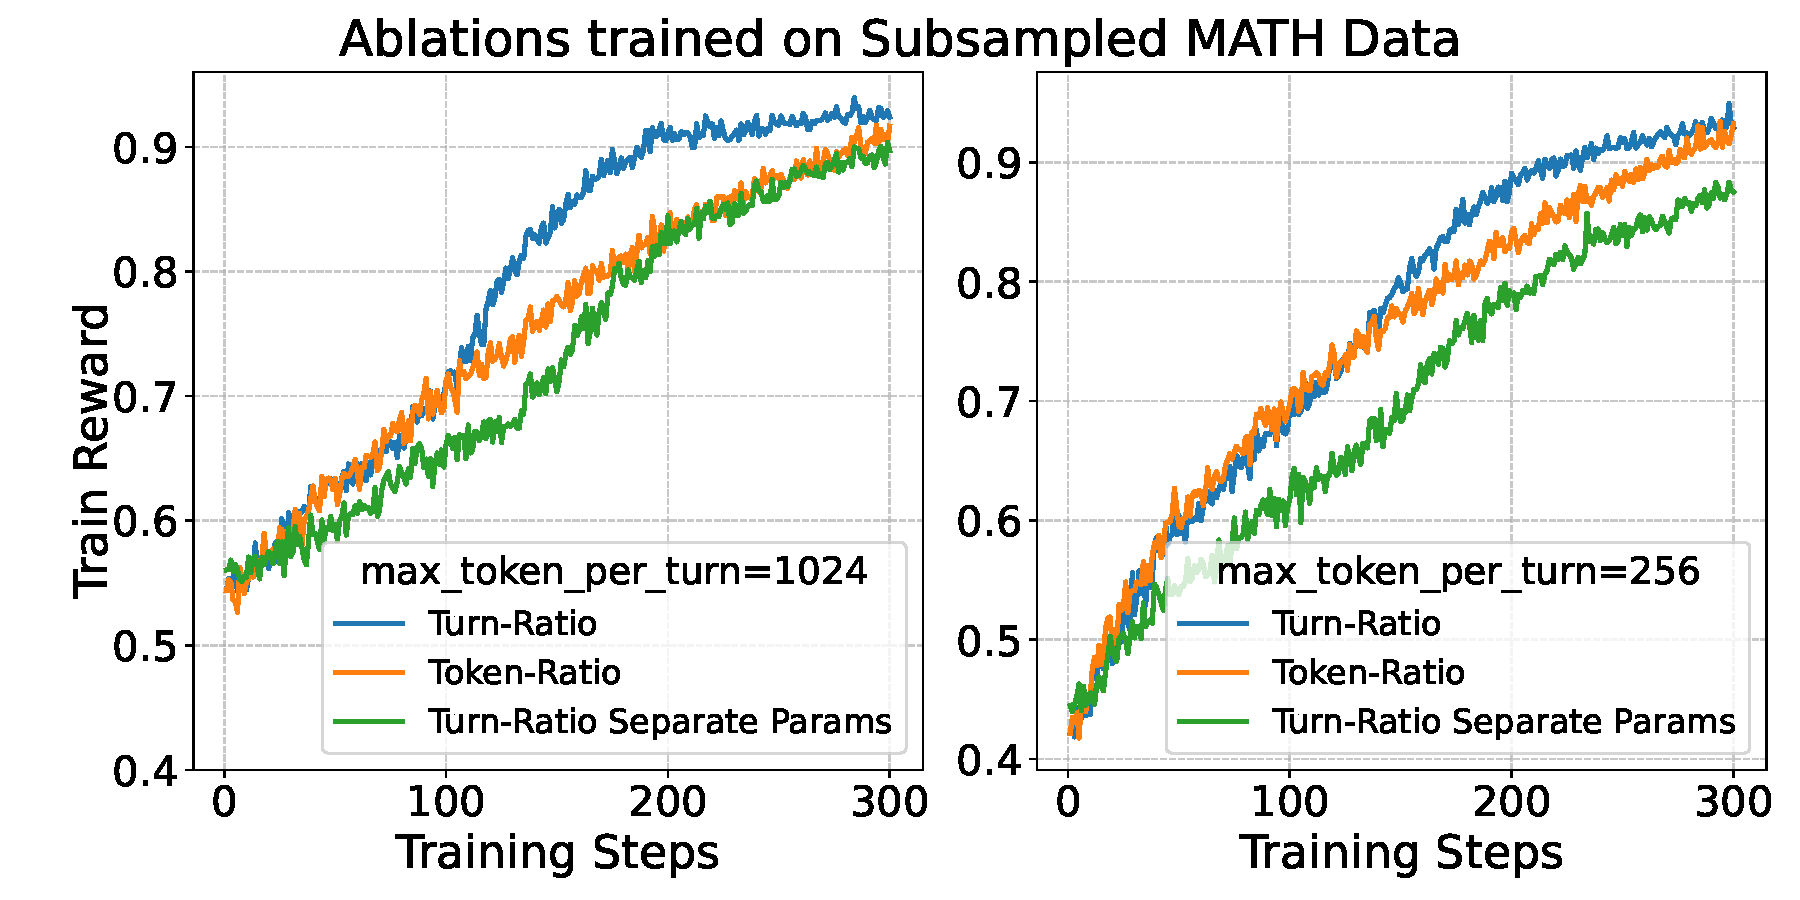
\includegraphics[width=\linewidth]{figures/multi_turn/multi_turn_ablation.pdf}
%         \vspace{-10pt}
%         \caption{Ablations of multi-turn ReMA on subset of MATH, we only show here the training curves of different settings.}
%         \label{fig:multi_turn_ablation}
%     \end{subfigure}
%     \vspace{-5pt}
%     \caption{Training Result of Multi-turn MAMRP in \method}
% \end{figure}

\subsubsection{Results and Ablations}
\label{sec:exp.multiturn.results}
\textbf{Question 4.} \textit{Can \method~be scaled to multi-turn settings?}

There are two key points revealed by our multi-turn ReMA experiments, as shown in Fig.~\ref{fig:multi_turn_main}. 
On one hand, \textbf{the algorithm can demonstrate effective convergence on the training set}, with accuracy steadily increasing from approximately 55\% to 70\% during training. 
It also achieves an average performance gain of about 5\% across all seven test benchmarks, indicating stable improvements on out-of-distribution data. (Experiment with the rollout config of \textit{turn30\_token512}, see Appendix~\ref{app:exp_setting.multi_turn_rema.math} and Fig.~\ref{fig:detailed_training_curves_2x4} for more details.)

On the other hand, we observe that the performance of multi-turn ReMA is highly sensitive to hyperparameters such as the maximum response length per turn and the maximum number of turns. 
For certain configurations, the model either collapses into producing massive repetitions within a single turn or generates empty responses after only a few turns. 
Similar phenomena have been reported in concurrent works such as RAGEN~\citep{wang2025ragen}, where these issues are attributed to the lack of fine-grained, reasoning-aware guidance. As a result, multi-turn RL becomes susceptible to long-horizon credit assignment challenges and state drift, often leading to reduced exploration diversity—a phenomenon referred to as the ``Echo Trap''. 
To address this challenge, it is essential to comprehensively explore the training recipe w.r.t. model, data, and algorithm.

% In our multi-turn ReMA experiments, we explore two key questions: first, whether the algorithm can converge on the training set, and second, whether it can achieve stable improvements on test sets. As presented in Figure~\ref{fig:multi_turn_main}, the accuracy on the training set gradually increases from approximately 55\% to 70\% , while achieve about 10\% performance gains averaged over all 7 test benchmarks. 

% Nonetheless, we find that multi-turn ReMA is extremely sensitive to parameters such as the setting of max response length in each round and the max number of turns.
% Both an excessively large max number of turns and an overly small per‑round token constraint can lead to collapse. As REGAN~\cite{wang2025ragen} pointed out, due to the lack of fine‑grained and reasoning‑aware guidance, multi-turn GRPO is prone to failure under long-horizon credit assignment and state drift in stochastic dynamics. And it often comes with the declines of exploration diversity, termed by "Echo Trap".

% \wxy{NOT SURE: We believe that, when necessary, adding fresh training data and increasing the token budget could be crucial for sustaining continued performance gains.}

% This indicates that the multi-turn interaction between agents enables more effective problem-solving capabilities. 
% The consistent improvement on out-of-distribution test sets is particularly encouraging, as it demonstrates the generalization capabilities of multi-turn ReMA.
% This suggests that the meta-thinking skills learned through multi-turn agent interactions transfer well to more challenging mathematical problems beyond the training distribution.
% This suggests that the meta-thinking skills acquired via multi-turn agent interactions can generalize to and improve performance on mathematical problems that are more challenging or out-of-distribution compared to the training data.

% \subsubsection{Ablations}
% \label{sec:exp.multiturn.ablation}
% To better understand the effectiveness of different design choices in multi-turn ReMA, we conduct several ablation studies as shown in Figure~\ref{fig:multi_turn_ablation}. We specifically compare different clipping settings (trajectory loss with turn-level clipping versus other approaches) and shared parameter update versus separated parameter update for the agents. For these experiments, we use a smaller dataset consisting of 133 samples in total (19 samples from each of the 7 problem types) to evaluate sample efficiency and convergence properties.
\textbf{Question 5.} \textit{How does parameter sharing and turn-level ratio affect multi-turn ReMA?}

As shown in Fig.~\ref{fig:multi_turn_ablation}, we compare different configurations on a smaller dataset consisting of 133 samples---19 from each of the 7 MATH problem types---to evaluate sample efficiency and convergence speed.
First, all configurations eventually achieve nearly 100\% accuracy on the training dataset. Notably, \textbf{the trajectory-level loss with turn-level ratio (\textit{Turn-Ratio}, Eq.~(\ref{eq:turn_grpo})) demonstrates substantially better sample efficiency} than its token-level variants (Eq.~(\ref{eq:grpo})), reaching higher training rewards with fewer steps.
% While the two approaches are theoretically expected to have similar convergence rates, 
We also present the training curve of separate weight setting, the empirical results show that \textbf{shared parameters with simultaneous updates converge noticeably faster}.